%% Example GayaUKM thesis in English
\documentclass[english]{GayaUKM}

\usepackage{graphicx}

\title{<Your Thesis Title>}
\author{<Your Name>}
\authorid{<P00000 ID No.>}
\faculty{<Your Faculty>}
\submissiondate{2 October 2013}
\submissionyear{2013}
\degreetype{Doctor of Philosophy}
\campus{Bangi}

\begin{document}

\maketitle

\frontmatter
\declaration

% Acknolwedgements from ack.tex
\begin{acknowledgements}
Thanks to all who have helped.
\end{acknowledgements}

% English abstract from abstract-en.tex
% Tajuk tesis dalam Bahasa Inggeris perlu diberikan.
\begin{enAbstract}[<Your English Title here>]
This is the English abstract. Auto single-line spacing. Jelly dessert sesame snaps. Oat cake jelly oat cake gingerbread sweet roll apple pie muffin sesame snaps. Dragée icing carrot cake faworki tart chocolate cake. Cookie apple pie chupa chups tootsie roll sweet roll toffee chocolate bar gummies gummi bears. Apple pie lollipop candy canes jujubes caramels. Soufflé powder liquorice fruitcake. Tiramisu fruitcake candy canes jelly beans muffin chupa chups bonbon. Donut sugar plum fruitcake liquorice chocolate pastry lollipop chocolate bar cookie. Jelly-o donut marshmallow chupa chups danish. Sugar plum pudding sweet roll muffin applicake biscuit tart fruitcake wafer. Pudding croissant carrot cake tiramisu candy canes. Powder powder jelly-o. Pie croissant cake chocolate cake carrot cake sweet apple pie sweet roll donut.
\end{enAbstract}

% Malay Abstract from abstrak-ms.tex
% The Malay translation of your title needs to be given here
\begin{msAbstract}[<Terjemahan Tajuk Tesis dalam Bahasa Melayu>]
Inilah abstrak dalam Bahasa Melayu. Data korpus merupakan data bahasa
Melayu yang datangnya dalam dua bentuk sumber, iaitu bentuk tulisan
dan bentuk lisan. Bentuk tulisan seperti buku, majalah, surat khabar,
makalah, monograf, dokumen, kertas kerja, efemeral, puisi, drama,
kad bahan, surat, risalah dan sebagainya. Sementara bentuk lisan yang
ditranskripsikan seperti ucapan, wawancara, temu bual, perbualan dan
sebagainya dalam pelbagai bentuk rakaman.
\end{msAbstract}



\tableofcontents
\listoffigures
\listoftables

% List of Symbols may be prepared as in symbols.tex
\chapter{List of Symbols}
\begin{center}
\doublespacing
\begin{tabular}{ll}
$b, c$ & constants\\
$C_f$ & local friction coefficient\\
\end{tabular}
\end{center}


\mainmatter
% Each chapter from a separate file
\chapter{Introduction}
\label{chap:intro}

\section{What is Lorem Ipsum?}
\label{sec:apadia}

Lorem Ipsum is simply dummy text of the printing and typesetting industry. Lorem Ipsum has been the industry's standard dummy text ever since the 1500s, when an unknown printer took a galley of type and scrambled it to make a type specimen book \cite{banerjee:pedersen:2003}. It has survived not only five centuries, but also the leap into electronic typesetting, remaining essentially unchanged. It was popularised in the 1960s with the release of Letraset sheets containing Lorem Ipsum passages, and more recently with desktop publishing software like Aldus PageMaker including versions of Lorem Ipsum \cite{berment:phd:2004}.



\section{Where Does It Come From?}
\label{sec:where}

The pressure coefficient for an incompressible fluid is given by
\begin{equation}
C_p = \frac{P - P_\infty}{\frac{1}{2} \rho {U_\infty}^2}
 = 1 - \left( \frac{U_1}{U_\infty} \right)^2,
\end{equation}
where $P$ is the local static pressure, $P_\infty$ is the static pressure at the beginning of the inlet section ($x = 0$ m) and $U_1$ and $U_\infty$ are the local and inlet free stream velocities, respectively. Figure 1(b) shows the $C_p$ distribution for the APG and FPG cases. The test section is configured such that a ZPG ($C_p = 0 \pm 0.01$) is maintained until $x \approx 3$ m, from which point a constant pressure gradient is maintained for both non-ZPG cases.

Contrary to popular belief, Lorem Ipsum is not simply random text. It has roots in a piece of classical Latin literature from 45 BC, making it over 2000 years old. Richard McClintock, a Latin professor at Hampden-Sydney College in Virginia, looked up one of the more obscure Latin words, consectetur, from a Lorem Ipsum passage, and going through the cites of the word in classical literature, discovered the undoubtable source \cite{azarova:etal:2002,budanitsky:hirst:2006}. Lorem Ipsum comes from sections 1.10.32 and 1.10.33 of ``de Finibus Bonorum et Malorum'' (The Extremes of Good and Evil) by Cicero, written in 45 BC. This book is a treatise on the theory of ethics, very popular during the Renaissance. The first line of Lorem Ipsum, ``''Lorem ipsum dolor sit amet\ldots'', comes from a line in section 1.10.32.

The standard chunk of Lorem Ipsum used since the 1500s is reproduced below for those interested. Sections 1.10.32 and 1.10.33 from ``de Finibus Bonorum et Malorum'' by Cicero are also reproduced in their exact original form, accompanied by English versions from the 1914 translation by H. Rackham. 

\begin{equation}
-\frac{(x_0 - \mu)^2}{2 \sigma^2} = -\ln 2
\end{equation}


\section{Examples}
\label{sec:examples}

The first few paragraphs of Lorem Ipsum are given below.

\subsection{First Paragraph}

Lorem ipsum dolor sit amet, consectetur adipiscing elit. Donec posuere, neque quis feugiat egestas, quam sapien dictum justo, eu vulputate nunc metus sed dui. Integer molestie leo quis libero facilisis, dictum pretium quam ornare. Vestibulum ante ipsum primis in faucibus orci luctus et ultrices posuere cubilia Curae; Vivamus luctus rutrum magna non convallis. Praesent vestibulum consequat eros, et fringilla nisi suscipit id. Nam vulputate justo dui, eu rutrum est accumsan ut. Sed molestie erat vitae mi blandit, in volutpat urna lobortis. Vestibulum mollis rutrum gravida. Fusce dolor nulla, condimentum vel pretium ut, venenatis eget leo. Ut semper placerat mauris, ut tempus est tempor vel. Interdum et malesuada fames ac ante ipsum primis in faucibus. In vitae feugiat diam. Pellentesque accumsan consequat turpis aliquam elementum.


\subsection{Next Two Paragraphs}

Vivamus dignissim arcu nunc, non aliquam sem porta vitae. Sed sodales accumsan dui sit amet egestas. Maecenas rhoncus a erat eget accumsan. 

\begin{table}[hbt!]\centering
\caption{Number of Jewels}

\begin{tabular}{l c}
\hline
Type & Quantity \\\hline
Sapphire & 6\\
Diamond & 23\\
Gold & 56\\
Silver & 235\\
Bronze & 324\\\hline
\end{tabular}
\end{table}

\begin{itemize}
\item Etiam vitae pulvinar metus, sed fringilla orci. 
\item Duis dapibus dolor risus, non ultrices enim porta sit amet. 
\item Ut eu libero augue. 
\end{itemize}

Nulla ipsum augue, feugiat ac laoreet quis, pretium ut magna. Class aptent taciti sociosqu ad litora torquent per conubia nostra, per inceptos himenaeos. Integer blandit placerat dictum.

\begin{figure}[hbt!]\centering

\includegraphics[width=.5\textwidth]{green}
\caption{Example figure}
\end{figure}

Sed dolor justo, scelerisque sed rutrum quis, porttitor a mauris. Cras non auctor felis, rutrum fringilla risus. Integer at convallis erat, sit amet luctus turpis. Duis sed rutrum eros, quis tempus risus. Etiam pellentesque nisi odio, eget dignissim eros ultrices et. Aliquam leo massa, fermentum vel odio sed, ullamcorper molestie lorem. Integer lorem felis, adipiscing sit amet interdum eget, auctor at lorem. Aliquam ultricies tortor eu nibh facilisis tincidunt.


\subsubsection{Some Notes}

Duis sed rutrum eros, quis tempus risus. Etiam pellentesque nisi odio, eget dignissim eros ultrices et. Aliquam leo massa, fermentum vel odio sed, ullamcorper molestie lorem.

\subsubsection{And Further}
Duis sed rutrum eros, quis tempus risus. Etiam pellentesque nisi odio, eget dignissim eros ultrices et. Aliquam leo massa, fermentum vel odio sed, ullamcorper molestie lorem.


\subsection{Least-Squares with Forgetting Factor AdaptiveLaw}

\section{Mechatronic Suspension System; History and a Brief Background}
Nulla ipsum augue, feugiat ac laoreet quis, pretium ut magna. Class aptent taciti sociosqu ad litora torquent per conubia nostra, per inceptos himenaeos. Integer blandit placerat dictum.



\section{Summary}
Nulla ipsum augue, feugiat ac laoreet quis, pretium ut magna. Class aptent taciti sociosqu ad litora torquent per conubia nostra, per inceptos himenaeos. Integer blandit placerat dictum.

Sed dolor justo, scelerisque sed rutrum quis, porttitor a mauris. Cras non auctor felis, rutrum fringilla risus. Integer at convallis erat, sit amet luctus turpis. Duis sed rutrum eros, quis tempus risus. Etiam pellentesque nisi odio, eget dignissim eros ultrices et. Aliquam leo massa, fermentum vel odio sed, ullamcorper molestie lorem. Integer lorem felis, adipiscing sit amet interdum eget, auctor at lorem. Aliquam ultricies tortor eu nibh facilisis tincidunt.
\chapter{Fibonacci Numbers}

In mathematics, the Fibonacci numbers or Fibonacci series or Fibonacci sequence are the numbers in the following integer sequence:
%
\begin{equation*} % example of unnumbered equations
0, 1, 1, 2, 3,5,8,13,21,34,55,89,144,\ldots
\end{equation*}

By definition, the first two numbers in the Fibonacci sequence are 0 and 1, and each subsequent number is the sum of the previous two. In mathematical terms, the sequence $F_n$ of Fibonacci numbers is defined by the recurrence relation
%
\begin{equation}
F_n = F_{n-1} + F_{n-2},
\end{equation}
%
with seed values
%
\begin{equation}
F_0 = 0, F_1 = 1.
\end{equation}

The Fibonacci sequence is named after Leonardo Fibonacci. His 1202 book Liber Abaci introduced the sequence to Western European mathematics, although the sequence had been described earlier in Indian mathematics. \cite{Goonatilake:1998} By modern convention, the sequence begins either with $F_0 = 0$ or with $F_1 = 1$. The Liber Abaci began the sequence with $F_1 = 1$, without an initial 0.


\section{Origins}

The Fibonacci sequence appears in Indian mathematics, in connection with Sanskrit prosody. \cite{Singh:1985} In the Sanskrit oral tradition, there was much emphasis on how long (L) syllables mix with the short (S), and counting the different patterns of L and S within a given fixed length results in the Fibonacci numbers; the number of patterns that are m short syllables long is the Fibonacci number $F_{m + 1}$.
\citet{Goonatilake:1998} writes that the development of the Fibonacci sequence ``is attributed in part to Pingala (200 BC), later being associated with Virahanka (c.~700 AD), Gopala (c.~1135), and Hemachandra (c.~1150)''.

\begin{figure}[hbt!]
\centering
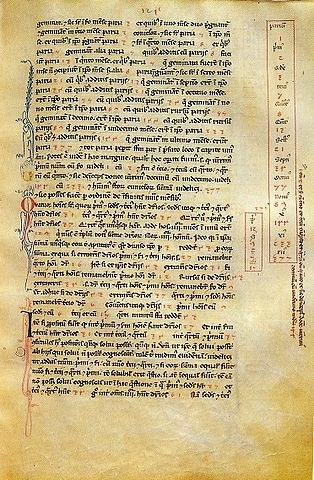
\includegraphics[width=.4\textwidth]{314px-Liber-abbaci-magliab-f124r}
\caption{A page of Fibonacci's Liber Abaci a very long title. This a very long title, just to test hanging captions.
%% DO NOT LEAVE BLANK LINES HERE
\source{Heinz L\"{u}neburg, Leonardi Pisani Liber Abaci oder Lesevergn\"{u}gen eines Mathematikers}
}
\end{figure}

\section{List of Fibonacci Numbers}

The first 11 Fibonacci numbers $F_n$ for $n = 0, 1, 2, \ldots, 10$ are:

\begin{table}[hbt!]\centering
\caption{First 11 Fibonacci Numbers for $n=0,1,\ldots$}
\begin{tabular}{|c|c|c|c|c|c|c|c|c|c|c|}
\hline
$F_0$ & $F_1$ & $F_2$ & $F_3$ & $F_4$ & $F_5$ & $F_6$ & $F_7$ & $F_8$ & $F_9$ & $F_{10}$\\
\hline
0 & 1 & 1 & 2 & 3 & 5 & 8 & 13 & 21 & 34 & 55 \\
\hline
\end{tabular}
\end{table}

The sequence can also be extended to negative index n using the re-arranged recurrence relation
%
\begin{equation}
F_{n-2} = F_n - F_{n-1},
\end{equation}
%
which yields the sequence of ``negafibonacci'' numbers satisfying
%
\begin{equation}
F_{-n} = (-1)^{n+1} F_n.
\end{equation}
%
Thus the bidirectional sequence is
\begin{table}[hbt!]\centering
\caption{Bidirectional Fibonacci Numbers sequence}
\begin{tabular}{|c|c|c|c|c|c|c|c|c|c|c|}
\hline
$F_{-5}$ & $F_{-4}$ & $F_{-3}$ & $F_{-2}$ & $F_{-1}$ & $F_0$ & $F_1$ & $F_2$ & $F_3$ & $F_4$ & $F_5$ \\\hline
5 & $-3$ & 2 & $-1$ & 1 & 0 & 1 & 1 & 2 & 3 & 5\\\hline
\end{tabular}
\end{table}

\citet{Rohl:1989} gives an account of how Fibonacci numbers can be computed efficiently.

\section{Applications}

\subsection{In Computation}

Fibonacci numbers have wide applications in mathematics as well as computer science:

\begin{itemize}
\item The Fibonacci numbers are important in the computational run-time analysis of Euclid's algorithm to determine the greatest common divisor of two integers: the worst case input for this algorithm is a pair of consecutive Fibonacci numbers.

\item Yuri Matiyasevich was able to show that the Fibonacci numbers can be defined by a Diophantine equation, which led to his original solution of Hilbert's tenth problem.

\item The Fibonacci numbers are also an example of a complete sequence. This means that every positive integer can be written as a sum of Fibonacci numbers, where any one number is used once at most.

\item Moreover, every positive integer can be written in a unique way as the sum of one or more distinct Fibonacci numbers in such a way that the sum does not include any two consecutive Fibonacci numbers. This is known as Zeckendorf's theorem, and a sum of Fibonacci numbers that satisfies these conditions is called a Zeckendorf representation. The Zeckendorf representation of a number can be used to derive its Fibonacci coding.

\item Fibonacci numbers are used by some pseudorandom number generators.

\item Fibonacci numbers are used in a polyphase version of the merge sort algorithm in which an unsorted list is divided into two lists whose lengths correspond to sequential Fibonacci numbers -- by dividing the list so that the two parts have lengths in the approximate proportion $\varphi$. A tape-drive implementation of the polyphase merge sort was described in The Art of Computer Programming.

\item Fibonacci numbers arise in the analysis of the Fibonacci heap data structure.

\item The Fibonacci cube is an undirected graph with a Fibonacci number of nodes that has been proposed as a network topology for parallel computing.

\item A one-dimensional optimization method, called the Fibonacci search technique, uses Fibonacci numbers.

\item The Fibonacci number series is used for optional lossy compression in the IFF 8SVX audio file format used on Amiga computers. The number series compands the original audio wave similar to logarithmic methods such as $\mu$-law.

\item Since the conversion factor 1.609344 for miles to kilometers is close to the golden ratio (denoted $\varphi$), the decomposition of distance in miles into a sum of Fibonacci numbers becomes nearly the kilometer sum when the Fibonacci numbers are replaced by their successors. This method amounts to a radix 2 number register in golden ratio base $\varphi$ being shifted. To convert from kilometers to miles, shift the register down the Fibonacci sequence instead.
\end{itemize}


\subsection{In Nature}

Fibonacci sequences appear in biological settings, in two consecutive Fibonacci numbers, such as branching in trees, arrangement of leaves on a stem, the fruitlets of a pineapple, the flowering of artichoke, an uncurling fern and the arrangement of a pine cone, and the family tree of honeybees. However, numerous poorly substantiated claims of Fibonacci numbers or golden sections in nature are found in popular sources, e.g.,~relating to the breeding of rabbits in Fibonacci's own unrealistic example, the seeds on a sunflower, the spirals of shells, and the curve of waves.

A model for the pattern of florets in the head of a sunflower was proposed by H.~Vogel in 1979. \cite{Vogel:1979} This has the form
\begin{equation}
\theta = \frac{2\pi}{\phi^2} n,\  r = c \sqrt{n}
\end{equation}
where $n$ is the index number of the floret and $c$ is a constant scaling factor; the florets thus lie on Fermat's spiral.

\begin{figure}[hbt!]\centering
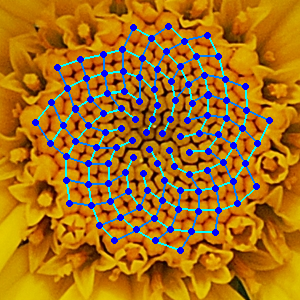
\includegraphics[width=.5\textwidth]{FibonacciChamomile}

\caption{Yellow Chamomile head}
\end{figure}

\chapter{Golden Ratio}

In mathematics and the arts, two quantities are in the golden ratio if their ratio is the same as the ratio of their sum to the larger of the two quantities, i.e.~their maximum. The figure on the right illustrates the geometric relationship. Expressed algebraically, for quantities $a$ and $b$ with $a > b$,
\begin{equation}
 \frac{a+b}{a} = \frac{a}{b} \ \stackrel{\text{def}}{=}\ \varphi,
\end{equation}
where the Greek letter $\varphi$ represents the golden ratio. Its value is:
\begin{equation}
\varphi = \frac{1+\sqrt{5}}{2} = 1.61803\,39887\ldots.
\end{equation}

\section{History}

Ancient Greek mathematicians first studied what we now call the golden ratio because of its frequent appearance in geometry. The division of a line into ``extreme and mean ratio'' (the golden section) is important in the geometry of regular pentagrams and pentagons. Euclid's Elements  provides the first known written definition of what is now called the golden ratio: ``A straight line is said to have been cut in extreme and mean ratio when, as the whole line is to the greater segment, so is the greater to the less.'' Euclid explains a construction for cutting (sectioning) a line ``in extreme and mean ratio'', i.e., the golden ratio. (See Figure~\ref{fig:line:golden}.) Throughout the Elements, several propositions (theorems in modern terminology) and their proofs employ the golden ratio.

\begin{figure}[hbt!]\centering
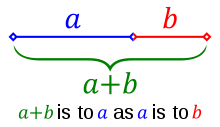
\includegraphics[width=.3\textwidth]{220px-Golden-ratio-line}
\caption{Line segments in the golden ratio}
\label{fig:line:golden}
\end{figure}

\begin{figure}[hbt!]\centering
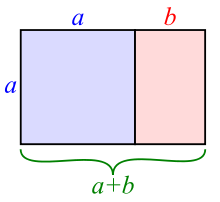
\includegraphics[width=.3\textwidth]{SimilarGoldenRectangles}
\caption{Golden rectangles}
\end{figure}



\section{Calculation}
Two quantities $a$ and $b$ are said to be in the golden ratio $\varphi$ if:
\begin{equation}
 \frac{a+b}{a} = \frac{a}{b} = \varphi.
\end{equation}

One method for finding the value of $\varphi$ is to start with the left fraction. Through simplifying the fraction and substituting in $\frac{b}{a} = \frac{1}{\varphi}$,
\begin{equation}
\frac{a+b}{a} = 1 + \frac{b}{a} = 1 + \frac{1}{\varphi},
\end{equation}

By definition, it is shown that
\begin{equation}
 1 + \frac{1}{\varphi} = \varphi. 
\end{equation}
Multiplying by $\varphi$ gives
\begin{equation*}
\varphi + 1 = \varphi^2
\end{equation*}
which can be rearranged to
\begin{equation*}
{\varphi}^2 - \varphi - 1 = 0.
\end{equation*}
Using the quadratic formula, two solutions are obtained:
\begin{equation*}
\varphi = \frac{1 + \sqrt{5}}{2} = 1.61803\,39887\dots
\end{equation*}
and
\begin{equation*}
\varphi = \frac{1 - \sqrt{5}}{2} = -0.6180\,339887\dots
\end{equation*}
Because $\varphi$ is the ratio between positive quantities $\varphi$ is necessarily positive:
\begin{equation*}
\varphi = \frac{1 + \sqrt{5}}{2} = 1.61803\,39887\dots .
\end{equation*}

Different representations of the golden ratio are given in Table~\ref{tab:goldenratio}.

\begin{table}[hbt!]\centering
\caption{Number representations of the golden ratio}
\label{tab:goldenratio}

\begin{tabular}{|l|l|}
\hline
Form & Representation\\\hline
Binary & 1.1001111000110111011\ldots\\\hline
Decimal & 1.6180339887498948482\ldots\\\hline
Hexadecimal	& 1.9E3779B97F4A7C15F39\ldots\\\hline
Continued fraction & $1 + \cfrac{1}{1 + \cfrac{1}{1 + \cfrac{1}{1 + \cfrac{1}{1 + \ddots}}}}$\\[6ex]\hline
Algebraic form & $\displaystyle\frac{1 + \sqrt{5}}{2}$\\[2ex]\hline
Infinite series & $\displaystyle\frac{13}{8}+\sum_{n=0}^{\infty}\frac{(-1)^{(n+1)}(2n+1)!}{(n+2)!\,n!\,4^{(2n+3)}}$\\[2ex]\hline
\end{tabular}
\end{table}




% references are listed in refs.bib
\bibliography{refs}

\appendix
% Each appendix chapter from a separate file
\chapter{Details}

Lorem ipsum dolor sit amet, consectetur adipiscing elit. Donec posuere, neque quis feugiat egestas, quam sapien dictum justo, eu vulputate nunc metus sed dui. Integer molestie leo quis libero facilisis, dictum pretium quam ornare. Vestibulum ante ipsum primis in faucibus orci luctus et ultrices posuere cubilia Curae; Vivamus luctus rutrum magna non convallis. Praesent vestibulum consequat eros, et fringilla nisi suscipit id. Nam vulputate justo dui, eu rutrum est accumsan ut. Sed molestie erat vitae mi blandit, in volutpat urna lobortis. Vestibulum mollis rutrum gravida. Fusce dolor nulla, condimentum vel pretium ut, venenatis eget leo. Ut semper placerat mauris, ut tempus est tempor vel. Interdum et malesuada fames ac ante ipsum primis in faucibus. In vitae feugiat diam. Pellentesque accumsan consequat turpis aliquam elementum.
\chapter{Software Code}

Lorem ipsum dolor sit amet, consectetur adipiscing elit. Donec posuere, neque quis feugiat egestas, quam sapien dictum justo, eu vulputate nunc metus sed dui. Integer molestie leo quis libero facilisis, dictum pretium quam ornare. Vestibulum ante ipsum primis in faucibus orci luctus et ultrices posuere cubilia Curae; Vivamus luctus rutrum magna non convallis. Praesent vestibulum consequat eros, et fringilla nisi suscipit id. Nam vulputate justo dui, eu rutrum est accumsan ut. Sed molestie erat vitae mi blandit, in volutpat urna lobortis. Vestibulum mollis rutrum gravida. Fusce dolor nulla, condimentum vel pretium ut, venenatis eget leo. Ut semper placerat mauris, ut tempus est tempor vel. Interdum et malesuada fames ac ante ipsum primis in faucibus. In vitae feugiat diam. Pellentesque accumsan consequat turpis aliquam elementum.
\end{document}